
\nsecbegin{Ziel des Sprints}
Es soll eine funktionsfähige Basisversion, welche für das einfache erstellen von Klassendiagrammen aus Java-Code verwendet werden soll entstehen. Das Programm soll sowohl über die Kommandozeile, als auch über eine grafische Oberfläche bedient werden können. Die erzeugten Klassendiagramme sollen in der grafischen Oberfläche angezeigt werden können.

\begin{figure}[hbtp]
\centering
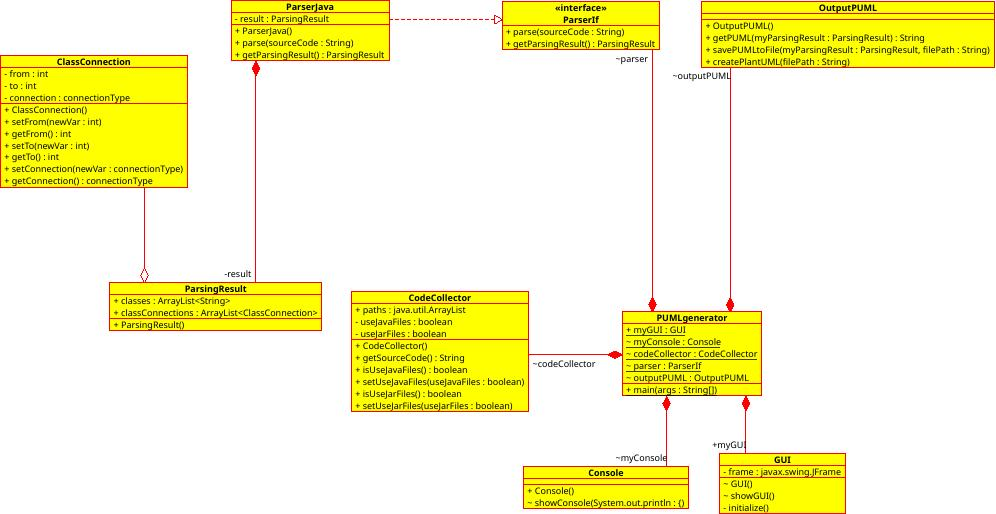
\includegraphics[scale=0.5]{Bilder/classDiagrammSprint1}
\caption{Klassendiagramm des Sprints}
\end{figure}
\nsecend

\nsecbegin{User-Stories des Sprint-Backlogs}
\nsecbegin{Dateien einlesen}
\nsecbegin{Art der eingelesenen Datei}
Als Benutzer wünsche ich mir, dass eine Auswahl zwischen Jar- und Java-Dateien möglich ist, damit Quellcode nicht doppelt eingelesen wird.
\nsecend

\nsecbegin{Java-Dateien}
Als Benutzer wünsche ich mir, dass Java-Dateien einlesbar sind, um den Quellcode von einer oder mehreren Klassen zu analysieren.
\nsecend

\nsecbegin{Jar-Dateien}
Als Benutzer wünsche ich mir, dass Jar-Dateien einlesbar sind, um den Quellcode zu analysieren.
\nsecend
\nsecend

\nsecbegin{Vorschau}
Als Benutzer wünsche ich mir eine Vorschau der Diagramme, damit ich einschätzen kann ob ich damit zufrieden bin.
\nsecend

\nsecbegin{Kommandozeile}
Als Benutzer wünsche ich mir, dass das Programm von der Kommandozeile aus aufrufbar ist, um es automatisiert starten zu können.
\nsecend

\nsecbegin{Klassendiagramme}
Als Benutzer wünsche ich mir, Klassendiagramme aus meinem bestehenden Quellcode erstellen zu können, damit ich das nicht manuell tun muss.
\nsecend

\nsecbegin{Anzeigen und Speichern von PlantUML}
Als Benutzer wünsche ich mir, Diagramme als PlantUML-Code anzeigen und speichern zu können, um den Aufbau nachvollziehen zu können.
\nsecend

\nsecbegin{Plattformunabhängigkeit}
Als Project Owner wünsche ich mir, dass das Programm plattformunabhängig ist, damit es sich gut verbreiten lässt.
\nsecend
\nsecend % {User-Stories des Sprint-Backlogs}

\nsecbegin{Zeitliche Planung}
\begin{figure}[hbtp]
\centering
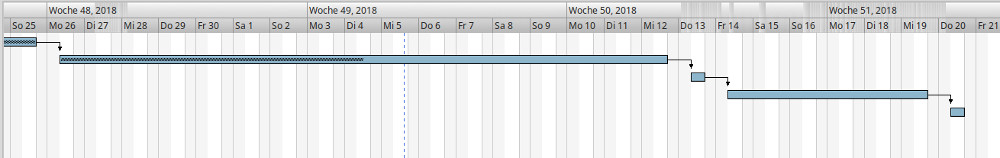
\includegraphics[width=\textwidth]{Bilder/gantt}
\caption{Gantt-Diagramm für Sprint 1}
\end{figure}
\nsecend

\nsecbegin{Liste der durchgeführten Meetings}
\begin{itemize}
\item Planning-Meeting (29.11.2018)
\item Zwischen-Meeting (03.12.2018)
\item Review-Meeting (13.12.2018)
\end{itemize}
\nsecend

\nsecbegin{Ergebnisse des Planning-Meetings}
Dem gesammten Team ist die geplante Grundstruktur des Programms bekannt. Jeder weis welchen Teil des Programms er implementieren soll.
\nsecend

\nsecbegin{Aufgewendete Arbeitszeit pro Person$+$Arbeitspaket}
\begin{longtable}{|p{4cm}|l|l|l|l|l|}
        \hline
        Arbeitspaket & Person & Start & Ende & h & Artefakt\\
        \hline
        Dummyklassen & Musterstudi & 3.5.09 & 12.5.09 & 14 & Klasse.java\\ \hline
        AP XYZ &  &  &  & & \\ \hline
\end{longtable}     
\nsecend

\nsecbegin{Konkrete Code-Qualität im Sprint}
XXX
\nsecend

\nsecbegin{Konkrete Test-Überdeckung im Sprint}
XXX
\nsecend

\nsecbegin{Ergebnisse des Reviews}
\begin{table}[H]

\begin{tabularx}{\textwidth}{ |l|l|X| }
\hline
\textbf{Klasse} & \textbf{Methode} & \textbf{Anmerkungen}\\
 \hline
Console & showConsole & Pfad anpassen \\
CodeCollector & - & Unit-Tests für Ordner \\
CodeCollector & getSourceCode & gleichzeitig .jar- und .java-Dateien \\
ParserJava & parse & Bug: Entfernt zu viel Source Code! Mehr Tests\\
OutputPuml & - & generell mehr Kommentare \\
OutputPuml & getPuml & Redundanter Code mit savePumlToFile, generell mehr Kommentare\\
OutputPuml & createPlantUML & Performance verbessern \\
GUI\_SWT & - & Entwicklerdokumentation (Installationsanleitung) für verwendetes Tool\\
\hline
\end{tabularx}
\end{table}

Sonstiges:
\begin{itemize}
\item mehr Kommentare
\item (Graphviz muss installiert sein, um PlantUML anzuzeigen)
\item Javadocs schreiben!
\item in gitconfig Name und Mail-Adresse anpassen! Wichtig für Benotung!
\item Ordner für Unit-Tests ist srcTest
\item im Ordner srcTest ein Unterordner "'testfiles"' ertellen, in dem zusätzliche Testdateien landen
\end{itemize}
\nsecend

\nsecbegin{Ergebnisse der Retrospektive}
XXX
\nsecend

\nsecbegin{Abschließende Einschätzung des Product-Owners}
XXX
\nsecend

\nsecbegin{Abschließende Einschätzung des Software-Architekten}
XXX
\nsecend

\nsecbegin{Abschließende Einschätzung des Team-Managers}
XXX
\nsecend

